\chapter{第一性原理计算及相关理论}\label{chap:first}
在过去的十到二十年间,计算物理已经发展成为一门独立的学科,与理论物理和实验物理呈“三足鼎立”之势。计算物理已经在包括生物学、化学、天体物理学、加速器物理学、固体物理学等诸多领域发挥着重要的作用。在凝聚态领域中,计算物理实际上是一门通过数值方法求解固体中原子分子特性的学科。其关键是表征物质的电子结构信息,即能带结构。
电子能带理论是基于量子力学和统计力学的理论方法。而密度泛函理论则是凝聚态物理中计算电子能带结构的主要理论基础。密度泛函理论的发展使计算物理能够成为连接理论和实验的桥梁,使得计算物理学家能够先于理论和实验物理准确预测一些材料可能的物性,并为实验物理提供研究的平台。基于密度泛函理论发展起来的第一性原理计算(First-Principles calculations),也称为从头计算($\textit{ab initio}$ calculations)的方法,仅需要知道所研究材料的基本信息,如原子结构和组分信息,不需要引入额外的经验参数,就可以使用现有的软件包求解出材料的电子结构,输运性质,热力学性质等,极大的推动了材料物理近几年的发展。其中,我们组在拓扑材料方面预言的拓扑绝缘体Bi$_2$Se$_3$,ZrTe$_5$,狄拉克半金属Na$_3$Bi,Cd$_3$As$_2$,外尔半金属TaAs和节线半金属ZrSiS都先于实验,并迅速将拓扑领域的研究推向高潮。
我们知道第一性原理计算研究离不开软件包的发展,目前成熟的第一性原理软件包有VASP,Wien2K,Openmx,Quantum Espresso,BSDATE等。

瓦尼尔函数方法是在第一性原理计算基础上发展出来的一套数值计算方法,将倒空间的布洛赫函数转化到实空间的瓦尼尔函数,利用实空间哈密顿量进行一系列计算。这个方法的优势是计算量小,速度快,尤其对于处理表面态的性质非常方便,因此也成为目前与第一性原理计算相辅相成的一个非常流行的工具。本章将首先介绍密度泛函理论的发展过程,然后能带理论的重要定理布洛赫定理,最后介绍瓦尼尔函数的一些基本性质。
%和kp模型一起,构成凝聚态计算物理分析物性的三大工具。本章首先将详细介绍密度泛函理论的发展,仅接着将在第一性原理计算基础上发展出来的一套瓦尼尔(Wannier)函数方法,最后介绍一种解析理解能带性质的$\mathbf{k}\cdot \mathbf{p}$方法。

\section{密度泛函理论}
密度泛函理论(DFT)的基本思想是多体相互作用粒子系统的任何性质都可以看作是基态密度$\rho(\vec{r})$的函数。这个证明最早是由Hohenberge和Kohn及Mermin的工作提出来的~\citep{Hohenberg1964,Mermin65}。Kohn-Sham设想将一个多体相互作用的问题用一个自由粒子问题加上考虑多体效应的交换关联函数来代替。下面我们将从描述多粒子体系的哈密顿量出发,一步步介绍如何推导得到DFT理论的基本方程(Kohn-Sham方程) 。 

我们从电子和原子核满足的基本哈密顿量出发,
\begin{equation}
    \label{eq:2-1}
    \begin{aligned}
    \hat{H}&=\hat{H}_e+\hat{H}_N+\hat{H}_{eN}\\
    &=-\frac{\hbar^{2}}{2 m_{e}} \sum_{i} \nabla_{i}^{2}+\frac{1}{2} \sum_{i \neq j} \frac{e^{2}}{\left|\mathbf{r}_{i}-\mathbf{r}_{j}\right|} \\
    &-\sum_{I} \frac{\hbar^{2}}{2 M_{I}} \nabla_{I}^{2}+\frac{1}{2} \sum_{I \neq J} \frac{Z_{I} Z_{J} e^{2}}{\left|\mathbf{R}_{I}-\mathbf{R}_{J}\right|}+\sum_{i, I} \frac{Z_{I} e^{2}}{\left|\mathbf{r}_{i}-\mathbf{R}_{I}\right|}
    \end{aligned}
\end{equation}
上式子由三部分组成,分别为体系中电子,原子核及电子与原子核相互作用三部分。其中,电子部分又分为电子的动能项和电子-电子的相互作用,原子核部分分为原子核的动能项和原子核-原子核的相互作用。这是一个描述多体相互作用的哈密顿量。在实际体系中,每立方米对$i$和$j$的求和是$10^{29}$次方,以当前计算机的算力,是根本无法计算的。因此很有必要通过近似和简化,将其推广到自由粒子的方法。

\subsection{波恩-奥本海默近似}
在方程\ref{eq:2-1}中,直接去掉相互作用项$\hat{H}_{eN}$是不合理的,因为$\hat{H}_{eN}$与其他两项是同一量级的。而整个哈密顿量中唯一可以看作小量的是$\frac{1}{M_I}$。如果将关于核的质量这一项看作是无限小量,那么核的动能项就可以忽略\citep{martin_2004}。这个近似相当于认为原子核只在平衡位置附近振动,而电子则绝热地围绕原子核做高速运动。那么哈密顿量就可以分成两部分考虑,认为考虑电子运动时,原子核在其瞬时平衡位置上,而考虑核运动时,高速运动的电子则相当于一个均匀的背景。这就是著名的绝热近似或波恩-奥本海默(Born-Oppenheimer)近似\citep{Born1927},由波恩和奥本海默在1927年提出。这个近似事实上是非常好的近似,成为后来理解金属中的电子输运性质,绝缘体中极化子的形成,某些金属-绝缘体相变,超导体BCS理论的基础\citep{Born1927}。

多粒子哈密顿量(\ref{eq:2-1})满足的薛定谔方程可以写作:
\begin{equation}
    \label{eq:2-2}
    H \Psi(\mathbf{r}, \mathbf{R})=E \Psi(\mathbf{r}, \mathbf{R})
\end{equation}
经过波恩-奥本海默近似后,薛定谔方程(\ref{eq:2-2})的解就可以写成电子部分和原子核部分波函数的直积形式:
\begin{equation}
    \label{eq:2-3}
    \Psi(\mathbf{r}, \mathbf{R})=\chi(\mathbf{R}) \psi(\mathbf{r}, \mathbf{R})
\end{equation}
其中$\chi(\mathbf{R})$描述原子核的运动,原子核如同在势阱中运动;$\psi(\mathbf{r}, \mathbf{R})$描述电子的运动,认为原子核固定在某瞬时位置\citep{solid}。电子部分波函数$\psi(\mathbf{r}, \mathbf{R})$中原子核的瞬时位置$\mathbf{R}$作为参数出现,故在今后的讨论中略去。此时,原子核满足的薛定谔方程为:
\begin{equation}
    \label{eq:2-4}
    \left(\sum_{\alpha} \frac{\mathbf{P}_{\alpha}^{2}}{2 M_{\alpha}}+\frac{1}{2} \sum_{\alpha \neq \beta} v\left(\mathbf{R}_{\alpha}, \mathbf{R}_{\beta}\right)+\sum_{\alpha} v_{e}\left(\mathbf{R}_{\alpha}\right)\right)\chi(\mathbf{R})=E^I \chi(\mathbf{R})
\end{equation}
电子体系满足的薛定谔方程为:
\begin{equation}
    \label{eq:2-5}
    \left(\sum_{i} \frac{\mathbf{p}_{i}^{2}}{2 m_{e}}+\frac{1}{2} \sum_{i \neq j} \frac{e^{2}}{\left|\mathbf{r}_{i}-\mathbf{r}_{j}\right|}+\sum_{i} v\left(\mathbf{r}_{i}\right)\right)\psi(\mathbf{r}, \mathbf{R})=E\psi(\mathbf{r}, \mathbf{R})
\end{equation}
其中$v_{e}\left(\mathbf{R}_{\alpha}\right)$是电子对原子核的平均作用,$v\left(\mathbf{r}_{i}\right)$是原子核对电子的平均作用。固体材料的性质主要由电子决定,所以我们只关心电子满足的薛定谔方程(\ref{eq:2-5})。此时相对于体系的薛定谔方程(\ref{eq:2-2})已经得到了很大的简化。但是,我们可以看到无论是原子核还是电子满足的薛定谔方程都仍然是多体方程,对于实际求解的难度仍然很大。所以,还需要进一步的近似加以简化。

\subsection{哈特利-福特近似}
薛定谔方程(\ref{eq:2-5})的第二项是电子-电子之间的库仑相互作用,这一项的存在为计算带来了很大的难度。如果这一项不存在,即认为电子不受周围电子的束缚,只受到离子势的微扰相互作用,即变为单电子方程,极大的简化了计算。这就是近自由电子近似。但这种近似显然是粗糙的,因为忽略了与其同量级的相互作用。所以近自由电子近似的应用非常有限,只对一些简单金属,如铜,碱金属比较适用,这类材料往往具有球形的费米面。但这个近似对于引入费米面的概念非常重要。

在此基础上,哈特利(Hartree)提出了一种更为严格的处理方法\citep{hartree_1928},即将电子-电子之间复杂的库仑相互作用看作一种平均势。这时,满足电子薛定谔方程(\ref{eq:2-5})的解则可以表达为单个电子波函数的乘积形式,称为Hartree波函数:
\begin{equation}
    \label{eq:2-6}
    \psi(\mathbf{r})=\varphi_{1}\left(\mathbf{r}_{1}\right) \varphi_{2}\left(\mathbf{r}_{2}\right) \varphi_{3}\left(\mathbf{r}_{3}\right) \cdots \varphi_{N}\left(\mathbf{r}_{N}\right)
\end{equation}
这种近似下,取一组正交归一的$\varphi_{i}(\mathbf{r})$,计算能量的期望值$E$。为得到系统能量最小值,将$E$对$\varphi_{i}(\mathbf{r})$做变分,$E_{i}$作为拉格朗日乘子:
\begin{equation}
    \label{eq:2-7}
    \delta\left[E-\sum_{i} E_{i}\left(\left\langle\varphi_{i} \mid \varphi_{i}\right\rangle-1\right)\right]=0
\end{equation}

则得到每个单电子波函数满足单电子方程:
\begin{equation}
    \label{eq:2-8}
    \left(-\frac{\hbar^{2}}{2 m} \nabla^{2}+V(\mathbf{r})+e^{2} \sum_{i \neq i^{\prime}} \int d \mathbf{r}^{\prime} \frac{\left|\varphi_{i^{\prime}}\left(\mathbf{r}^{\prime}\right)\right|^{2}}{\left|\mathbf{r}^{\prime}-\mathbf{r}\right|}\right) \varphi_{i}(\mathbf{r})=E_{i} \varphi_{i}(\mathbf{r})
\end{equation}
第一项是电子动能项,第二项是单电子受到的晶格势,第三项是但电子受到其他电子的平均库仑势。拉格朗日乘子$E_{i}$有单电子能量的含义。可见,Hartree近似中,哈密顿量是严格,而波函数做了平均场近似。由于第三项的平均库仑势是单电子波函数的函数,所以求解这个薛定谔方程需要用自洽求解的方法。这部分详细讨论可参考:\cite{solid}。

电子是费米子,应当满足泡利不相容原理,即每个电子的量子态不同。这一点Hartree近似是满足的。但是Hartree近似忽略了电子之间的交换反对称性,即任意交换了两个位置的电子,应该产生一个负号。为了满足这个条件,福克(Fock)将单电子的波函数写成了Slater行列式的形式~\citep{Slater30,1930fock}:
\begin{equation}
    \label{eq:2-9}
    \psi(\mathbf{q})=\frac{1}{\sqrt{N !}}\left|\begin{array}{cccc}
    \varphi_{1}\left(q_{1}\right) & \varphi_{1}\left(q_{2}\right) & \cdots & \varphi_{1}\left(q_{N}\right) \\
    \varphi_{2}\left(q_{1}\right) & \varphi_{2}\left(q_{2}\right) & \cdots & \varphi_{2}\left(q_{N}\right) \\
    \vdots & \vdots & \ddots & \vdots \\
    \varphi_{N}\left(q_{1}\right) & \varphi_{N}\left(q_{2}\right) & \cdots & \varphi_{N}\left(q_{N}\right)
    \end{array}\right|
\end{equation}
其中,$\varphi_{i}$是位于$q_i$处的$i$个电子的波函数,$q_i$同时包含位置和自旋。这就是Hartree-Fock近似,也称为分子轨道近似或单行列式近似。再按照Hartree近似推导单电子方程相同的方法,对能量的期望值进行变分,就可以得到单电子的满足的Hartree-Fock方程:
\begin{equation}
    \label{eq:2-10}
    \begin{array}{c}
    \left(-\frac{\hbar^{2}}{2 m} \nabla^{2}+V(\mathbf{r})+e^{2} \sum_{i \neq i^{\prime}} \int d \mathbf{r}^{\prime} \frac{\left|\varphi_{i^{\prime}}\left(\mathbf{r}^{\prime}\right)\right|^{2}}{\left|\mathbf{r}^{\prime}-\mathbf{r}\right|}\right) \varphi_{i}(\mathbf{r}) \\
    -e^{2} \sum_{i \neq i^{\prime}, \|} \int d \mathbf{r}^{\prime} \frac{\varphi_{i^{\prime}}^{*}\left(\mathbf{r}^{\prime}\right) \varphi_{i}\left(\mathbf{r}^{\prime}\right)}{\left|\mathbf{r}^{\prime}-\mathbf{r}\right|} \varphi_{i^{\prime}}(\mathbf{r})=E_{i} \varphi_{i}(\mathbf{r})
    \end{array}
\end{equation}
Hartree-Fock方程在各种计算软件中被广泛采用,被认为是现代量子化学的基石。然而Hartree-Fock近似虽然考虑了电子之间的交换相互作用,但是却没有考虑自旋反平行电子的关联相互作用。所以对于关联相互作用比较强的体系,Hartree-Fock近似不再适用。


% \subsection{Koopmans定理}
% 总能量不是单粒子能量的和。

\subsection{托马斯-费米-狄拉克近似}
%\section{Thomas-Fermi-Dirac近似}
托马斯-费米(Thomas-Fermi)近似~\citep{thomas_1927,fermi_1927,dirac_1930}是密度泛函理论基本思想的来源。在1927年Thomas和Fermi最早的工作中,他们将电子的动能项看作是给定点的局域密度的函数,将系统的电子看作是均匀电子气中非相互作用的电子。他们忽略了电子之间的交换和关联作用。
1930年,狄拉克(Dirac)又将这个理论推广到考虑电子交换相互作用的情况~\citep{dirac_1930}。之后又有很多工作将这一理论推广到非均匀体系。尽管托马斯-费米-狄拉克近似很粗糙,不能足够精确的给出能带结构,但是其物理本质正是后来更为精确的密度泛函理论建立的基础。

\subsection{Hohenberg-Kohn定理}
Hohenberg和W.Kohn在研究非均匀电子气理论时提出两个定理\citep{Hohenberg1964},这使得密度泛函理论变为一个精确的多体理论,可以用于任何处于外势$V_{ext}$中相互作用电子的系统。密度泛函理论正是建立在这两个Hohenberg-Kohn定理之上~\citep{Hohenberg1964}:

定理一:不计自旋的全同费米子系统的基态能量是粒子数密度函数$\rho(\mathbf{r})$的唯一泛函。

定理二:能量泛函$E(\rho)$在粒子数不变条件下对正确的粒子数密度函数$\rho(\mathbf{r})$取极小值,并等于基态能量。

定理一的核心内容是说,决定系统基本物理性质的量是粒子数密度函数$\rho(\mathbf{r})$。定理二的核心内容是讲,在粒子数不变条件下能量泛函对于密度函数的变分就得到系统基态的能量$E_{G}[\rho]$。
对于N个电子相互作用的哈密顿量,可以写作:
\begin{equation}
    \label{eq:2-11}
    \begin{aligned}
    \hat{H}&=T+V_{ee}+V_{ext}\\
    &=-\frac{\hbar^{2}}{2 m_{e}} \sum_{i} \nabla_{i}^{2}+\frac{1}{2} \sum_{i \neq j} \frac{e^{2}}{\left|\mathbf{r}_{i}-\mathbf{r}_{j}\right|}+\sum_{i} V_{\mathrm{ext}}\left(\mathbf{r}_{i}\right)
    \end{aligned}
\end{equation}
第一项是动能项,第二项是电子之间的库仑相互作用,第三项是外势。根据定理一,我们首先将基态能量写成电荷密度泛函的形式:
\begin{equation}
    \label{eq:2-12}
    \begin{aligned}
    E(\rho, V) &=\left\langle\psi(\rho)\left|T+V_{e e}+V_{e x t}\right| \psi(\rho)\right\rangle\\
    &=T(\rho)+V_{e e}(\rho)+\int d^{3} \mathbf{r} V_{e x t}(\mathbf{r}) \rho(\mathbf{r}) \\
    &=T(\rho)+\frac{1}{2} \int d^{3} \mathbf{r} d^{3} \mathbf{r}^{\prime} \frac{\rho(\mathbf{r}) \rho\left(\mathbf{r}^{\prime}\right)}{\left|\mathbf{r}-\mathbf{r}^{\prime}\right|}+E_{x c}(\rho)+\int d^{3} \mathbf{r} V_{e x t}(\mathbf{r}) \rho(\mathbf{r}) 
    %\\& \equiv F(\rho)+\int d^{3} \mathbf{r} V_{e x t}(\mathbf{r}) \rho(\mathbf{r})
    \end{aligned}
\end{equation}
然后根据定理二,基态能量可以通过能量泛函对密度函数变分得到,即
\begin{equation}
    \label{eq:2-13}
    \int \mathrm{d} r \delta \rho(\boldsymbol{r})\left[\frac{\delta T[\rho(\boldsymbol{r})]}{\delta \rho(\boldsymbol{r})}+\int \mathrm{d} \boldsymbol{r}^{\prime} \frac{\rho\left(\boldsymbol{r}^{\prime}\right)}{\left|\boldsymbol{r}-\boldsymbol{r}^{\prime}\right|}+\frac{\delta E_{\mathrm{xc}}[\rho(\boldsymbol{r})]}{\delta \rho(\boldsymbol{r})}+V_{ext}(\boldsymbol{r})\right]=0
\end{equation}
上述方程中仍存在三个问题需要解决,就是如何确定$T[\rho]$,$\rho(\boldsymbol{r})$, $E_{\mathrm{xc}}[\rho]$。为了回答前两个问题,我们就必须要介绍著名的Kohn-Sham $\textit{AnSatz}$~\citep{Kohn-Sham,martin_2004}。

\subsection{Kohn-Sham \it{AnSatz}}
W.Kohn和L.J.Sham在1965年提出一个假设,即现在熟知的“Kohn-Sham $\textit{AnSatz}$”:假定非相互作用的“电子”体系与相互作用电子体系有相同的基态电荷密度~\citep{Kohn-Sham,martin_2004}。具体地,即假定未知的动能泛函$T[\rho]$可以由一个自由粒子的动能泛函$T_s[\rho]$来代替,将二者的差别放到复杂的交换关联函数$E_{\mathrm{xc}}[\rho]$中去。这个假设将一个复杂的多体问题转化为一个独立的单电子问题加上一个复杂的交换关联的问题。这意味着可以用处理自由粒子的方法来处理多体问题。
进一步,取
\begin{equation}
    \label{eq:2-14}
    \begin{array}{c}
    \rho(\boldsymbol{r})=\sum\limits_{i=1}^{N}\left|\varphi_{i}(\boldsymbol{r})\right|^{2} \\
    T_{\mathrm{s}}[\rho]=\sum\limits _{i=1}^{N} \int \mathrm{d} r \varphi_{i}^{*}(\boldsymbol{r})\left(-\nabla^{2}\right) \varphi_{i}(\boldsymbol{r})
    \end{array}
\end{equation}
则由方程\ref{eq:2-14}可得到单粒子满足的方程为:
\begin{equation}
    \label{eq:2-15}
    \left(-\frac{\hbar}{2 m} \nabla^{2}+V_{e x t}(\mathbf{r})+e^{2} \int d^{3}\ \mathbf{r}^{\prime} \frac{\rho\left(\mathbf{r}^{\prime}\right)}{\left|\mathbf{r}^{\prime}-\mathbf{r}\right|}+\frac{\delta E_{x c}(\rho)}{\delta \rho}\right) \varphi_{i}(\mathbf{r})=E_{i} \varphi_{i}(\mathbf{r})
\end{equation}
这就是著名的Kohn-Sham(KS)方程。由于这里的$\rho(\boldsymbol{r})$包含
$ \varphi_{i}$,因此需要自洽求解。后来的计算物理发展出很多处理复杂的交换关联函数的方法,包括局域密度近似(Local Density Approximation, LDA)~\citep{lda1,lda2}和广义梯度近似(Generalized Gradient Approximation, GGA)~\citep{gga1,gga2,pbe}。只要确定交换关联泛函的具体形式,就可以严格求解KS方程,从而得到基态能量,波函数以及其他物理量。
\begin{figure}[!t]
    \centering
    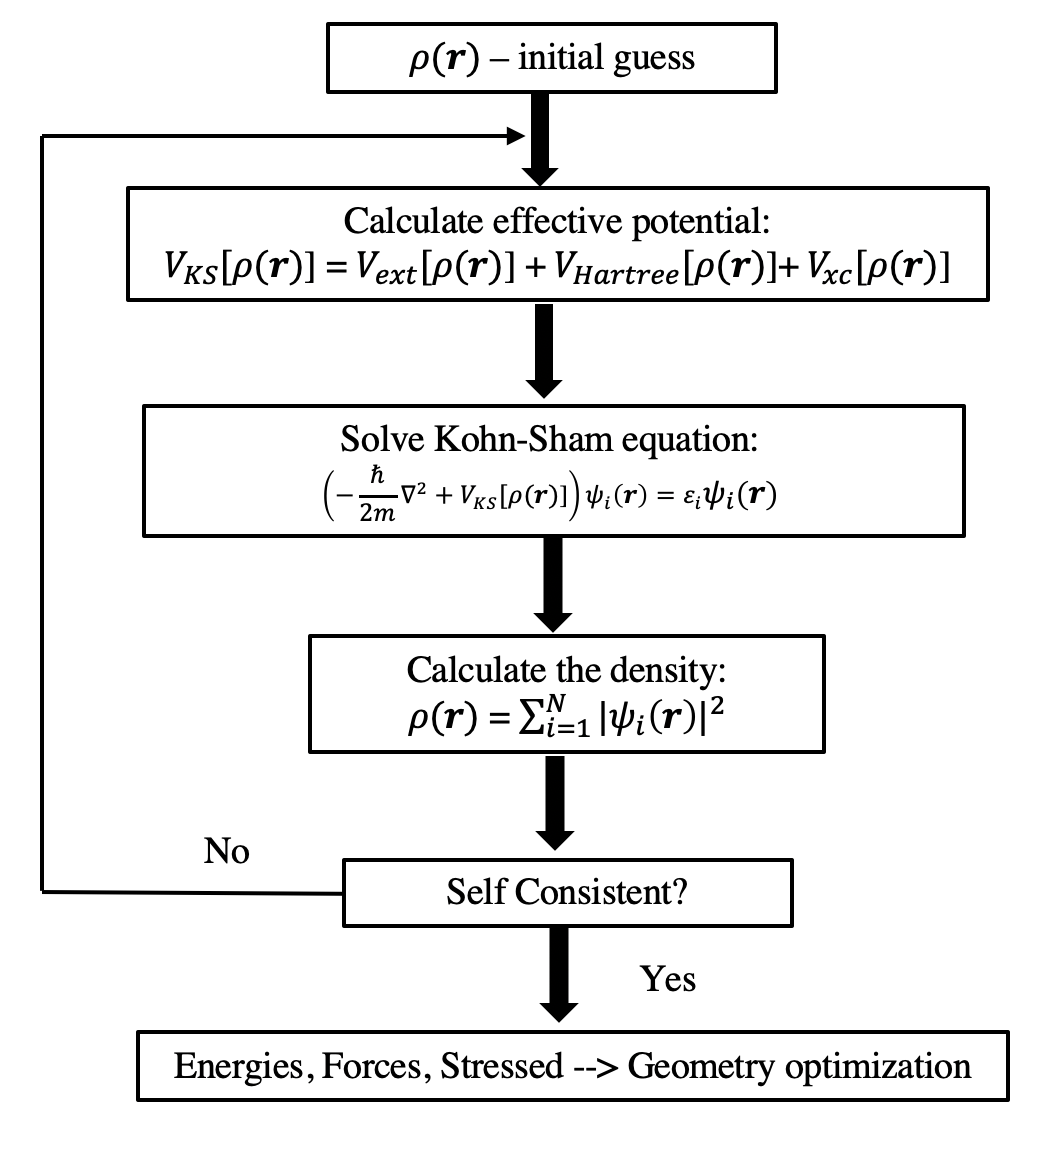
\includegraphics[width=10cm]{chapter2-1.png}
    \bicaption{自洽求解Kohn-Sham方程的流程图。(来自\citep{martin_2004})}{Flow chart of solving the self-consistent Kohn-Sham equation. (From~\citep{martin_2004})}
    \label{fig:2-1}
\end{figure}

自洽求解的流程图如图\ref{fig:2-1},先假设一个初始态密度,利用初始态密度和交换关联函数计算有效势,再带入到KS方程里求解波函数和总能,利用得到的波函数信息计算新的电荷密度,此时检验两个电荷密度是否自洽,如果不自洽就重复上述步骤,直至找到自洽的电荷密度,这样得到的电荷密度,波函数,基态能和其他物理量就是比较准确的。
\section{布洛赫定理及周期场近似}
电子受到的势场包括离子实对电子的势场和电子对电子对平均势场两部分。但是如果把固体看作是理想晶体,那么KS方程中的有效势$V_{eff}=V_{ext}(\mathbf{r})+e^{2} \int d \mathbf{r}^{\prime} \frac{\rho\left(\mathbf{r}^{\prime}\right)}{\left|\mathbf{r}^{\prime}-\mathbf{r}\right|}+V_{xc}(\rho[\mathbf{r})]$具有理想晶体的同样的平移对称性,也就是说它是个严格的周期势场。这个假设称之为周期场近似,或近自由电子近似。布洛赫定理(Bloch theorem)的内容是:

对于周期性势场,即$V(\mathbf{r})=\mathbf{r+R_n}$,其中$\mathbf{R_n}$是布拉维格子任意格矢,则单电子KS方程
\begin{equation}
    \label{eq:2-16}
    H \varphi_{n}(\boldsymbol{r})=\left[-\nabla^{2}+V_{\mathrm{KS}}(\boldsymbol{r})\right] \psi_{n}(\boldsymbol{r})=E_{n} \varphi_{n}(\boldsymbol{r})
\end{equation}
的本征函数是按照布拉维格子周期性调幅的平面波,满足:
\begin{equation}
    \label{eq:2-17}
    \begin{aligned}
    \varphi_{n}(\mathbf{k}, \mathbf{r})&=\mathrm{e}^{i \mathbf{k} \cdot \mathbf{r}} u_{n}(\mathbf{k}, \mathbf{r})\\
    u_{n}(\mathbf{k}, \mathbf{r})&=u_{n}\left(\mathbf{k}, \mathbf{r+R_{n}}\right).
    \end{aligned}
\end{equation}
其中,$\mathbf{k}$的物理意义是倒格矢。根据布洛赫定理,我们可以得到
\begin{equation}
    \label{eq:2-18}
    \begin{aligned}
    \varphi(\mathbf{r+R_{n}})=\mathrm{e}^{i \mathbf{k} \cdot \mathbf{r}} \varphi(\mathbf{r})
    \end{aligned}
\end{equation}
我们通常把满足方程\ref{eq:2-16}和方程\ref{eq:2-17}的函数称为布洛赫波函数。由于倒格矢$\mathbf{k}$具有周期性,所以求解薛定谔方程\ref{eq:2-16}只需要在一个不等价的$\mathbf{k}$区域(第一布里渊区)求解本征值,得到的便是每一个$\mathbf{k}$点给出的一系列分立的能谱$E_n(\mathbf{k})$,称之为能带。只要知道材料的能带信息,波函数信息,就可以进一步分析材料很多基本的物理性质,如拓扑性质、磁有序、光学性质、热导率、振动谱等等。能带理论无疑是凝聚态物理研究的支柱。本论文的工作正是基于固体能带理论来理解材料的拓扑性质。上述部分的详细讨论可以参考文献~\cite{solid,solid2,solid3}。
不同能带计算方法主要分为两类:一类是选择不同的基底展开晶体的布洛赫函数,包括平面波法、正交化平面波方法(orthogonalized plane-wave method, OPW)等;一类是对电子周期势作合理、有效的近似处理,这就是指我们常说的赝势。现在主要有三种赝势方法;模守恒赝势~\citep{Hamann1979,Hamann1989},超软赝势~\citep{soft90}和投影缀加平面波方法~\citep{paw1,paw2}。

\section{瓦尼尔函数}
周期运动的电子的本征函数是布洛赫函数,布洛赫函数是倒空间的周期函数。
%我们可以将布洛赫函数按照实空间基矢展开,展开系数称之为
与布洛赫函数不同,瓦尼尔函数(Wannier function)\citep{Wannier,wf1,wf2}是实空间的一组正交完备的局域函数。所以二者可以通过一个傅立叶变换联系起来。Wannier由于其有非常好的局域性而对于理解材料的电子结构和实际计算带来很大的方便。但是Wannier函数本身又有规范依赖的不确定性,因而为实际使用带来了困难。本节,我们将围绕这个不确定的相因子展开讨论。
% $\varphi_{i}^{\mathbf{k}}(\mathbf{r}) \rightarrow \tilde{\varphi}_{i}^{\mathbf{k}}(\mathbf{r})=\mathrm{e}^{\mathrm{i} \phi_{i}(\mathbf{k})} \varphi_{i}^{\mathbf{k}}(\mathbf{r})$
由布洛赫定理(方程\ref{eq:2-17}),我们知道$\varphi_{n}(\mathbf{k}, \mathbf{r})=\mathrm{e}^{i \mathbf{k} \cdot \mathbf{r}} u_{n}(\mathbf{k}, \mathbf{r})$。当做一个规范变换
$u_{n}^{\mathbf{k}}(\mathbf{r}) \rightarrow \tilde{u}_{n}^{\mathbf{k}}(\mathbf{r})=\mathrm{e}^{\mathrm{i} \phi_{i}(\mathbf{k})} u_{n}^{\mathbf{k}}(\mathbf{r})$,仍然是哈密顿量能量为$E(\mathbf{k})$的本征态。所以,以$\mathbf{R}$为中心的Wannier函数$w_{n\mathbf{R}}(\mathbf{r})$ 可以写作:
\begin{equation}
    \label{eq:2-19}
    w_{n \mathbf{R}}(\mathbf{r})=\frac{V}{(2 \pi)^{3}} \int_{\mathrm{BZ}}\left[\sum_{m} U_{m n}^{(\mathbf{k})} \varphi_{m \mathbf{k}}(\mathbf{r})\right] e^{-\mathrm{i} \mathbf{k} \cdot \mathbf{R}} \mathrm{d} \mathbf{k}
\end{equation}
其中布洛赫函数$U(1)$相因子在多带系统中则是幺正旋转矩阵$U_{m n}^{(\mathbf{k})}$,满足:
\begin{equation}
    \label{eq:2-20}
    u_{n \mathbf{k}}(\mathbf{r}) \rightarrow \sum_{m} U_{m n}(\mathbf{k}) u_{m \mathbf{k}}(\mathbf{r})
\end{equation}
由于$U_{m n}(\mathbf{k})$的不确定性导致Wannier函数的不确定性。那么如何才能得到最局域的Wannier函数呢?

\subsection{最局域的瓦尼尔函数}
为了得到最局域的Wannier函数,则需要最小化$U_{m n}(\mathbf{k})$。为此,定义一个Wannier函数的展宽函数$\Omega$:
\begin{equation}
    \label{eq:2-21}
    \Omega=\sum_{n}\left[\left\langle w_{n 0}(\mathbf{r})\left|r^{2}\right| w_{n 0}(\mathbf{r})\right\rangle-\left|\left\langle w_{n 0}(\mathbf{r})|\mathbf{r}| w_{n 0}(\mathbf{r})\right\rangle\right|^{2}\right]
\end{equation}
展宽函数$\Omega$又可以分为两部分,一部分是规范不变的$\Omega_I$,一部分是依赖于$U_{m n}(\mathbf{k})$的$U_{m n}(\mathbf{k})$的$\tilde{\Omega}$:
\begin{equation}
    \label{eq:2-22}
    \begin{array}{c}
    \Omega=\Omega_{\mathrm{I}}+\tilde{\Omega}=\Omega_{\mathrm{I}}+\Omega_{\mathrm{D}}+\Omega_{\mathrm{OD}} 
    \end{array}
\end{equation}
其中,
\begin{equation}
    \label{eq:2-23}
    \begin{array}{c}
    \Omega_{\mathrm{I}}=\sum\limits_{n}\left[\left\langle w_{n 0}(\mathbf{r})\left|r^{2}\right| w_{n 0}(\mathbf{r})\right\rangle-\sum\limits_{\mathbf{R} m}\left|\left\langle w_{n \mathbf{R}}(\mathbf{r})|\mathbf{r}| w_{n \mathbf{0}}(\mathbf{r})\right\rangle\right|^{2}\right] \\
    \Omega_{\mathrm{D}}=\sum\limits_{n} \sum\limits_{\mathbf{R} \neq 0}\left|\left\langle w_{n \mathbf{R}}(\mathbf{r})|\mathbf{r}| w_{n 0}(\mathbf{r})\right\rangle\right|^{2} \\
    \Omega_{\mathrm{OD}}=\sum\limits_{m \neq n} \sum\limits_{\mathbf{R}}\left|\left\langle w_{m \mathbf{R}}(\mathbf{r})|\mathbf{r}| w_{n 0}(\mathbf{r})\right\rangle\right|^{2}
    \end{array}
\end{equation}
这里$\Omega_D$和$\Omega_{OD}$分别是以Wannier函数为基矢的对角项和非对角项。
计算$\Omega$唯一需要的信息就是交叠矩阵:
\begin{equation}
    \label{eq:2-24}
    M_{m n}^{(\mathbf{k}, \mathbf{b})}=\left\langle u_{m \mathbf{k}} \mid u_{n, \mathbf{k}+\mathbf{b}}\right\rangle
\end{equation}
经过离散$k$空间,然后经过仔细推导\citep{wf1},可以得到如下形式:
\begin{equation}
    \label{eq:2-25}
    \Omega_{\mathrm{I}} =\frac{1}{N} \sum_{\mathbf{k}, \mathbf{b}} w_{b}\left(N-\sum_{m n}\left|M_{m n}^{(\mathbf{k}, \mathbf{b})}\right|^{2}\right)=\frac{1}{N} \sum_{\mathbf{k}, \mathbf{b}} w_{b} \operatorname{tr}\left[P^{(\mathbf{k})} Q^{(\mathbf{k}+\mathbf{b})}\right]
\end{equation}
%
\begin{equation}
    \label{eq:2-26}
    \Omega_{\mathrm{OD}}=\frac{1}{N} \sum_{\mathbf{k}, \mathbf{b}} w_{b} \sum_{m \neq n}\left|M_{m n}^{(\mathbf{k}, \mathbf{b})}\right|^{2} 
\end{equation}
%
\begin{equation}
    \label{eq:2-27}
    \Omega_{\mathrm{D}}=\frac{1}{N} \sum_{\mathbf{k}, \mathbf{b}} w_{b} \sum_{n}\left(-\operatorname{Im} (\ln M_{n n}^{(\mathbf{k}, \mathbf{b})})-\mathbf{b} \cdot \overline{\mathbf{r}}_{n}\right)^{2}
\end{equation}
其中$P^{(\mathbf{k})}=\Sigma_{n}\left|u_{n \mathbf{k}}\right\rangle\left\langle u_{n \mathbf{k}}\right|$, $Q^{(\mathbf{k})}=1-P^{(\mathbf{k})}$,能带指标$m,n$取值为$1,2,...,N$。从方程\ref{eq:2-25}显而易见,如果$\mathbf{k}$点和附近的$\mathbf{k+b}$点的波函数的交叠矩阵的平方越大,$\Omega_{\mathrm{I}}$越小。当两个波函数完全重叠时,这一项为零。所以$P^{(\mathbf{k})} Q^{(\mathbf{k}+\mathbf{b})}$代表的意思是$\mathbf{k}$点的子空间$\mathcal{S}$和$\mathbf{k+b}$点的子空间$\mathcal{S(\mathbf{k+b})}$ 子空间之间的“溢出”程度。
因此最小化$\Omega_I$的过程就是从一个由$N_k$条第一性原理计算的能带展开的$N_k$维的希尔伯特空间$\mathcal{F(k)}$中选出一个由$N$条Wannier轨道构成的$N$维子空间$\mathcal{S(\mathbf{k})}$的过程,在这个子空间中电子几乎局域,能带几乎光滑连接。实际计算中采用的方法就是不断迭代进行,直到达到最佳的“全局平滑度”。这个过程相对简单。

为了获得最局域化的Wannier函数,我们需要进一步优化$\tilde{\Omega}$。Marzari和Vanderbilt提出来的SMV算法\citep{wf2}就是最小化规范依赖的$\tilde{\Omega}$这一项。通过最小化$\tilde{\Omega}$,得到幺正变换矩阵$U_{m n}(\mathbf{k})$,满足
\begin{equation}
    \label{eq:2-28}
    u_{n \mathbf{k}}^{W}=\sum_{m=1}^{N_{\mathbf{k}}} U_{m n}(\mathbf{k}) u_{m \mathbf{k}}
\end{equation}
对$u_{n \mathbf{k}}^{W}$做傅立叶变换就可以得到实空间最局域的Wannier函数。同时对倒空间的哈密顿量做这个幺正变换,就得到此时的$H^W_{nm}(\mathbf{k})$。同样地,对$H^W_{nm}(\mathbf{k})$做傅立叶变换就得到实空间的哈密顿量$H^W_{nm}(\mathbf{R})$。$H^W_{nm}(\mathbf{R})$的物理意义就是在实空间基矢下不同轨道之间的跃迁。得到这个实空间哈密顿量的好处是对涉及实空间格子的处理的计算比较方便,比如表面态的计算,slab计算等。并且对哈密顿量进行处理相比于直接通过第一性原理计算的计算量大大降低,需要的计算资源更少,运算速度大大提高。

\subsection{原子轨道瓦尼尔函数}
我们发现在上述优化过程中没有对对称性有任何约束,这样得到的Wannier函数必然是破坏对称性的。这对于有对称性的晶体结构来讲,得到的能带信息就不准确,这对于分析材料的性质带来了困难。有两个思路来避免这个问题。一个思路是将上述得到的哈密顿量再进行后处理,进行强制对称化。具体操作的步骤就是让哈密顿量满足$
D(R) H\left(R^{-1} \mathbf{k}\right) D^{-1}(R)=H(\mathbf{k})
$,强制使两个由对称联系的矩阵元相等。这个方法已经有现成的软件包来做,但有时对于对称性很差的哈密顿量有时得不到理想的结果。

另一个思路就是直接构造满足对称性的Wannier函数。这个思路又包含两条可行的方法。一个方法是在对称性的限制下重新推导$U_{mn}(\mathbf{k})$~\citep{sakuma}。但这个计算过程比较复杂,对于自旋轨道耦合的体系又有收敛问题。第二个方法是直接构造原子轨道的Wannier函数。其实再上一节中,Marzari等优化$\Omega_I$的过程我们没有详细讨论,事实上具体操作步骤是先找到$N$个局域的试探轨道$\phi_n(\mathbf{r})$,然后投影到$N_k$个布洛赫本征态上,
\begin{equation}
    \label{eq:2-29}
    \left|\tilde{\psi}_{n \mathbf{k}}\right\rangle=\sum_{m=1}^{N_{\mathbf{k}}} A_{m n}\left|\psi_{m \mathbf{k}}\right\rangle
\end{equation}
其中$A_{m n}=\left\langle\psi_{m \mathbf{k}} \mid \phi_{n}\right\rangle$是$N_k \times N$维的投影矩阵。此时的$A_{mn}$就作为初始的$U_{mn}$矩阵,即
\begin{equation}
    \label{eq:2-30}
    \left|\psi_{n \mathbf{k}}^{W}\right\rangle=\sum_{m}\left| \psi_{m \mathbf{k}}\right\rangle \left\langle\psi_{m \mathbf{k}}\mid \phi_{n}\right\rangle=\sum_{m} U_{m n}(\mathbf{k})\left| \psi_{m \mathbf{k}}\right\rangle
\end{equation}
最后优化$U_{mn}$矩阵即可,而不再对$\tilde{\Omega}$进行优化。而选择原子轨道的好处是,我们可以限制原子轨道的Wannier函数满足晶体对称性,进而得到满足对称性的Wannier哈密顿量。对于考虑自旋轨道耦合的情况,我们可以分别对自旋上下进行计算,最后再加上自旋轨道耦合矩阵即可。

假设$\mathbf{k}$为简约布里渊区内一点,$\mathbf{k'}$由对称性操作$\hat{P}_{\{R \mid t\}}$与$\mathbf{k}$相联系,即$\mathbf{k'}=R\ \mathbf{k}$。经过仔细推导,我们会发现$\mathbf{k'}$点的交叠矩阵和投影矩阵满足,
\begin{equation}
    \begin{array}{r}
    A_{m n}^{\mathbf{k}}=\left\langle\psi_{m \mathbf{k}} \mid \phi_{\alpha}^{\mu}\right\rangle=\left\langle\hat{P}_{\{R \mid t\}} \psi_{m \mathbf{k}} \mid \hat{P}_{\{R \mid t\}} \phi_{\alpha}^{\mu}\right\rangle=\left\langle\psi_{m R \mathbf{k}} \mid \phi_{R \alpha}^{\mu^{\prime}}\right\rangle e^{-i(R \mathbf{k}) \cdot \mathbf{R}_{0}} \\
    M_{m n}^{\mathbf{k b}}=\left\langle u_{m \mathbf{k}} \mid u_{n \mathbf{k}+\mathbf{b}}\right\rangle=\left\langle\hat{P}_{\{R \mid t\}} e^{-i k \cdot r} \psi_{m \mathbf{k}} \mid \hat{P}_{\{R \mid t\}} e^{-i(k+b) \cdot r} \psi_{n \mathbf{k}+\mathbf{b}}\right\rangle \\
    =\left\langle e^{-i R \mathbf{k} \cdot t} u_{m, R \mathbf{k}} \mid e^{-i R(\mathbf{k}+\mathbf{b}) \cdot t} u_{n, R \mathbf{k}+\mathbf{b}}\right\rangle=M_{m n}^{R \mathbf{k}, R \mathbf{b}} e^{-i R \mathbf{b} \cdot t}
    \end{array}
\end{equation}
这样只要计算简约布里渊区内$\mathbf{k}$点的交叠矩阵$M_{m n}^{\mathbf{k b}}$和投影矩阵$A_{m n}^{\mathbf{k}}$,其他对称性相联系的$\mathbf{k'}$点的情况就可以由上式得到。通过这个方法,不仅可以得到保持对称性的Wannier函数,还可以提高运算速度。
%再通过L$\ddot{o}$wdin对称性正交化过程得到$N$个正交的轨道$\left|{\psi}^0_{n \mathbf{k}}\right\rangle$。最后再将这$N$个布洛赫函数转化为原胞周期函数$u^0_n(k)$


%\section{Wilson-loop方法}
%\section{{$\bold{k}$}\cdot {$\bold{p}$}微扰理论}

